%===============================================================================
% Terminals.
%===============================================================================

\section{Terminals}

%===============================================================================
\subsection{Terminal I/O Overview}

\begin{itemize}
\item Terminal is an input/output device.
\item You can read from and write to it.
\item Historicaly, it was a hardware device.
\begin{itemize}
	\item Connected to the computer via a serial line.
	\item There was no stderr as we know it now.
	\item A keyboard and a paper roll for displaying text (no video
	displays at the time).
	\item Then, video displays came in (AKA "glass TTYs").
\end{itemize}
\end{itemize}

\begin{itemize}
\item Whatever is displayed on the terminal comes from the terminal driver, ie.
what you type goes right over the serial line to the computer, the input might
be processed in a few different ways, and the output goes back to the terminal
to be displayed -- unless the echo is ``off''. \emsl{The terminal does not
display directly what you type, it always goes through the terminal driver code
running on the computer.}
\item Also note that RS-232, a commonly used standard for serial communication,
is a fully duplex protocol.
\end{itemize}

%===============================================================================
\subsection{Terminal I/O Overview (cont.)}

\begin{itemize}
\item today, a \emph{terminal} usually means a \emph{text terminal}, not a
\emph{physical terminal}
\begin{itemize}
	\item a text terminal usually runs under a graphical environment
\end{itemize}

\item some byte sequences have special meaning
\begin{itemize}
	\item moving the cursor, clearing the screen, etc.
	\item try \texttt{vim >output} and see what is in \texttt{output}
	\begin{itemize}
		\item do not forget to type ``:q'' as well
	\end{itemize}
\end{itemize}

\item different terminals have different capabilities
\begin{itemize}
	\item some cannot clear the screen, for example
	\item types of terminals: ansi, vt100, xterm, ...
\end{itemize}
\end{itemize}

\begin{itemize}
\item You probably know that we can also have virtual terminals on a console.
Most un{}ix-like system support that. Usually you can switch between virtual
terminals by hitting \texttt{Alt + Fx} where \texttt{Fx} is a function key.
	\begin{itemize}
	\item Virtual terminal configuration varies. On BSD systems, you have
	file \texttt{/etc/ttys} to set what virtual (and network) terminals you
	have.
	\end{itemize}
\item UNIX windowing (ie., graphical) environments did not eradicate the
terminal interface since it is very convenient to deal with.
\item Some applications might even refuse to run without a terminal -- screen
oriented editors, for example.
\item When running a terminal in the graphical environment, \texttt{xterm}, for
example, then that is the application that gets the keyboard input. It then
processes the input and sends the filtered data to the shell through a pseudo
terminal. Do not worry about pseudo terminals now, will be explained later.
\item You have to distinguish what is supported by the terminal, the terminal
driver itself, and what is done in the shell. For example, the terminal driver
offers by default \^{}D for ``End-Of-File'', meaning that it will close its
output (usually, shell's input) when \^{}D (binary \texttt{04}) is read
from the terminal, or \^{}S which suspends the output from the driver. However,
\texttt{bash} itself, for example, accepts \^{}L to clear the screen. That means
that \^{}L goes through the terminal and the terminal driver to the shell which
interprets it and sends a ``clear the screen'' sequence back to the terminal, if
the terminal itself supports the feature. \^{}L is not interpreted by the
terminal driver in contrast to \^{}D or \^{}S. More information is on page
\pageref{TERMIOS}.
\item When you hit \^{}C, that character is sent by the terminal application
(eg. \texttt{xterm}) which is interpreted by the terminal driver which generates
the \texttt{SIGINT} signal to the application. That means that neither the
terminal application nor the shell generates that signal. You can verify it like
this -- start \texttt{cat} in your shell. Then, \texttt{truss} your
\texttt{xterm} (not shell! Remember, \texttt{ptree} is great on Solaris for
finding out child-parent relationships. On Linux distros, try ``\texttt{ps
--forest}'') or any other terminal you use. Move your mouse to the terminal
again. You can press \texttt{Ctrl} itself several times to see that there is
some communication between the terminal and X over the X11 socket; use
\texttt{pfiles} to check which file descriptor is the X11 socket. Then, type
\^{}C. You should see something like this:

\begin{verbatim}
write(4, "03", 1)                               = 1
ioctl(3, FIONREAD, 0x08047A50)                  = 0
pollsys(0x080479D0, 2, 0x00000000, 0x00000000)  = 1
read(4, " ^ C", 1024)                           = 2
read(4, 0x08074C4A, 1022)                       Err#11 EAGAIN
\end{verbatim}

The terminal writes \texttt{03} to the terminal because that's what \^{}C is.
\texttt{03} means 1 byte of value 3. Note that \^{}E is \texttt{05} then, \^{}L
is \texttt{12} etc. Be careful that \texttt{truss} shows some characters using
escapes so \^{}J is $\backslash$\texttt{n} (\texttt{0A}, new line), \^{}L is
$\backslash$\texttt{f} (\texttt{0C}, form feed), and \^{}M is
$\backslash$\texttt{r} (\texttt{0D}, carriage return). What you get from the
terminal is literaly ``\^{}C'' in two characters, and that's what you see in
your terminal, literaly. Shell does not send it, that's the (pseudo) terminal
driver. More on this later.
\end{itemize}

%===============================================================================
\subsection{Physical (Hardware) Terminal}

\begin{center}
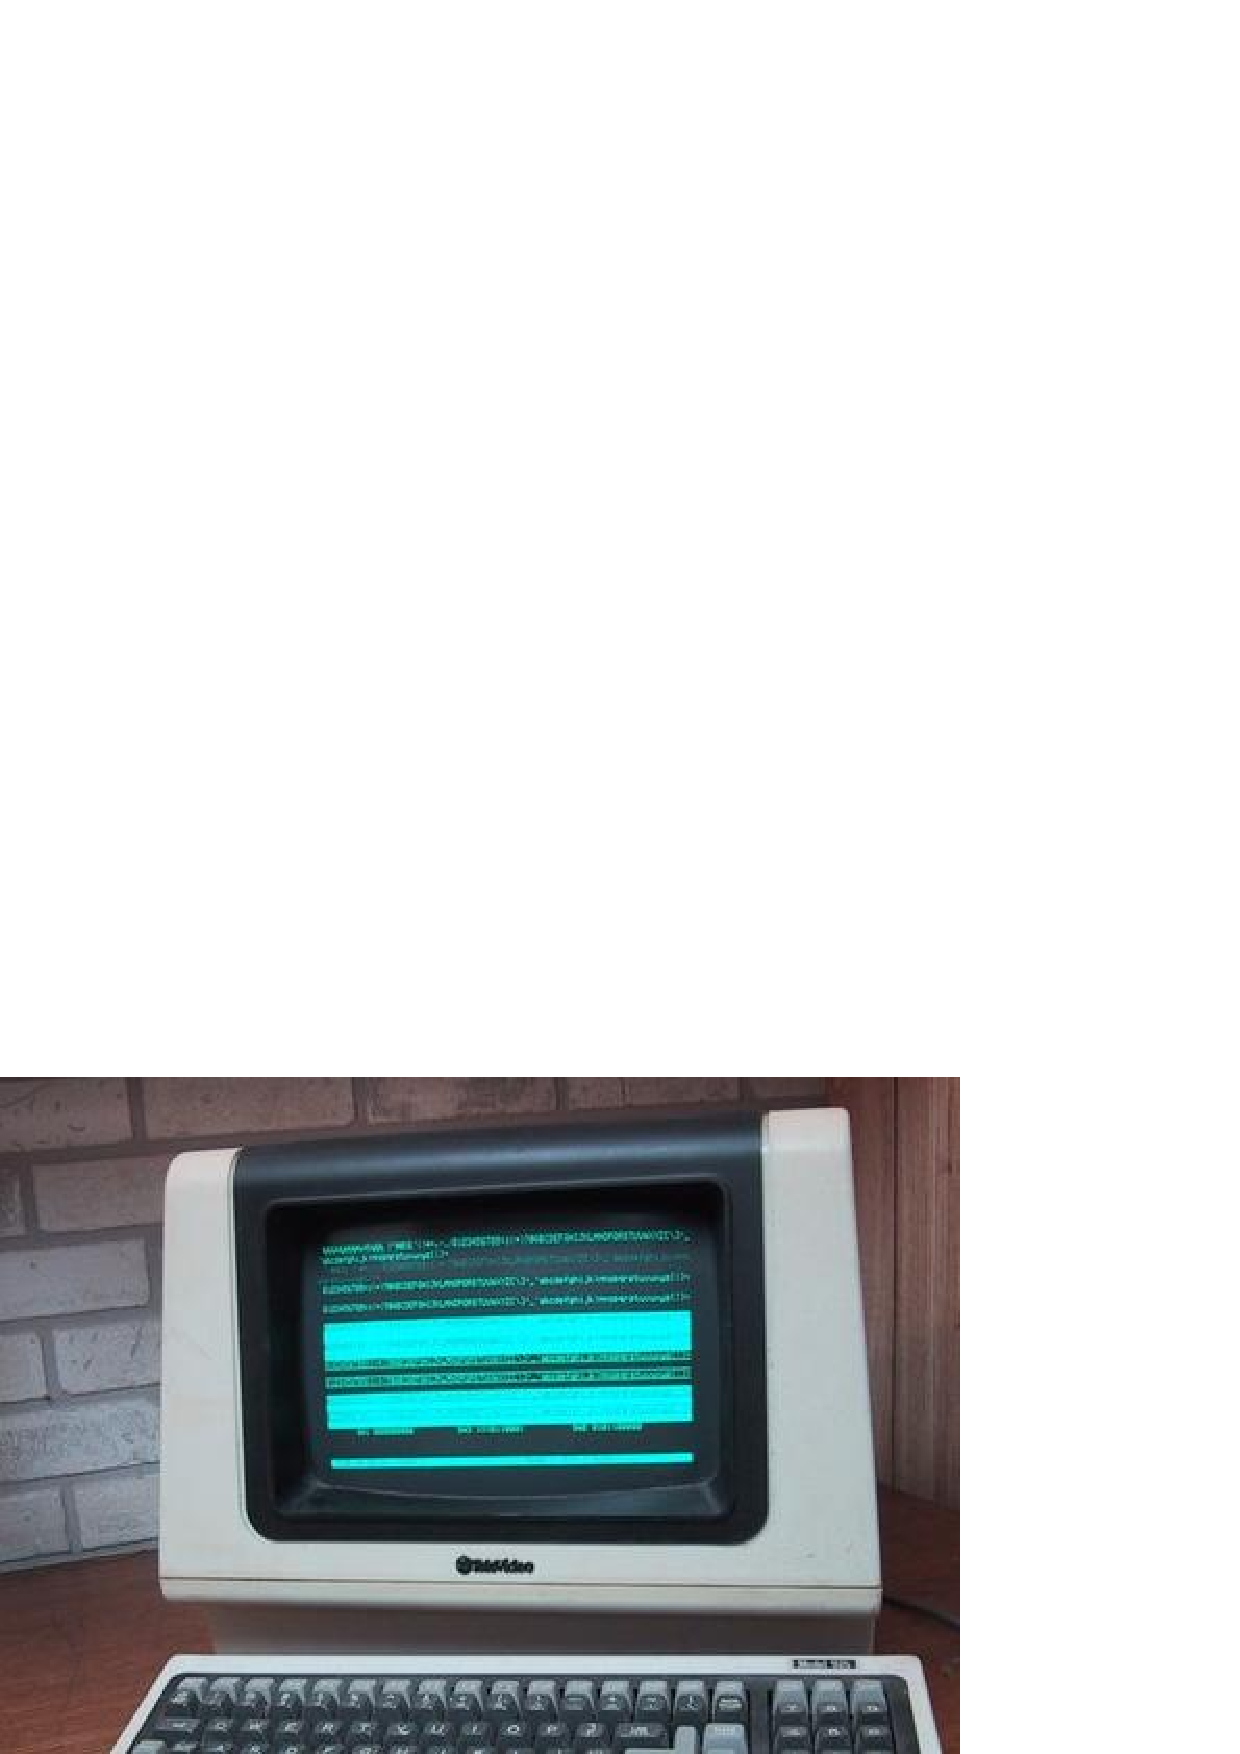
\includegraphics[width=90mm]{img/terminals/Televideo925Terminal.pdf}
\end{center}

\begin{itemize}
\item Picture in public domain downloaded from Wikipedia.
\item Note that while it looks like a ``normal'' computer it is not. It just
communicates with the ``real'' computer over a serial line.
\item As already mention, remember that echo (ie. what you see when you type) on
the terminal display is not done by the terminal itself. The terminal can output
only what it gets from the other side, meaning that the ``remote'' system (= the
terminal driver) itself does that echo for you. This can be switched off via the
\texttt{tcsetattr} function, which will be introduced later. You can use
"\texttt{stty -echo}" from the command line to switch off the echo, and
"\texttt{stty echo}" to switch it on again.
\item Even these days, you might need to use your computer to emulate a physical
terminal. Some devices like Cisco routers and switches might still need to be
configured with the IP address and the gateway using the serial console before
you can log it to it. You can use \texttt{tip(1)} (usually shipped by default
with your UNIX or un{}ix-like system) or myriad of other comms like
\texttt{Minicom} etc.
\end{itemize}

%===============================================================================
\subsection{\texttt{stty}(1) command}

\begin{itemize}
\item changes and prints the terminal line settings
\item \texttt{stty -a}
	\begin{itemize}
	\item lists the settings in a human readable form
	\end{itemize}
\item example
	\begin{itemize}
	\item \texttt{stty -echo} disables echo
	\item \texttt{stty echo} enables echo
	\end{itemize}
\item maybe most useful example of this command
	\begin{itemize}
	\item \texttt{stty sane}
	\item for example, if you paste some rubbish by mistake, and your
	terminal starts acting weird, the \texttt{sane} option often helps.
		\begin{itemize}
	  	\item not every time though
		\end{itemize}
	\end{itemize}
\end{itemize}

\begin{itemize}
\item We will use this command in other examples.
\end{itemize}


%===============================================================================
\subsection{TTY Driver Connected To a Phy Terminal}

\begin{center}
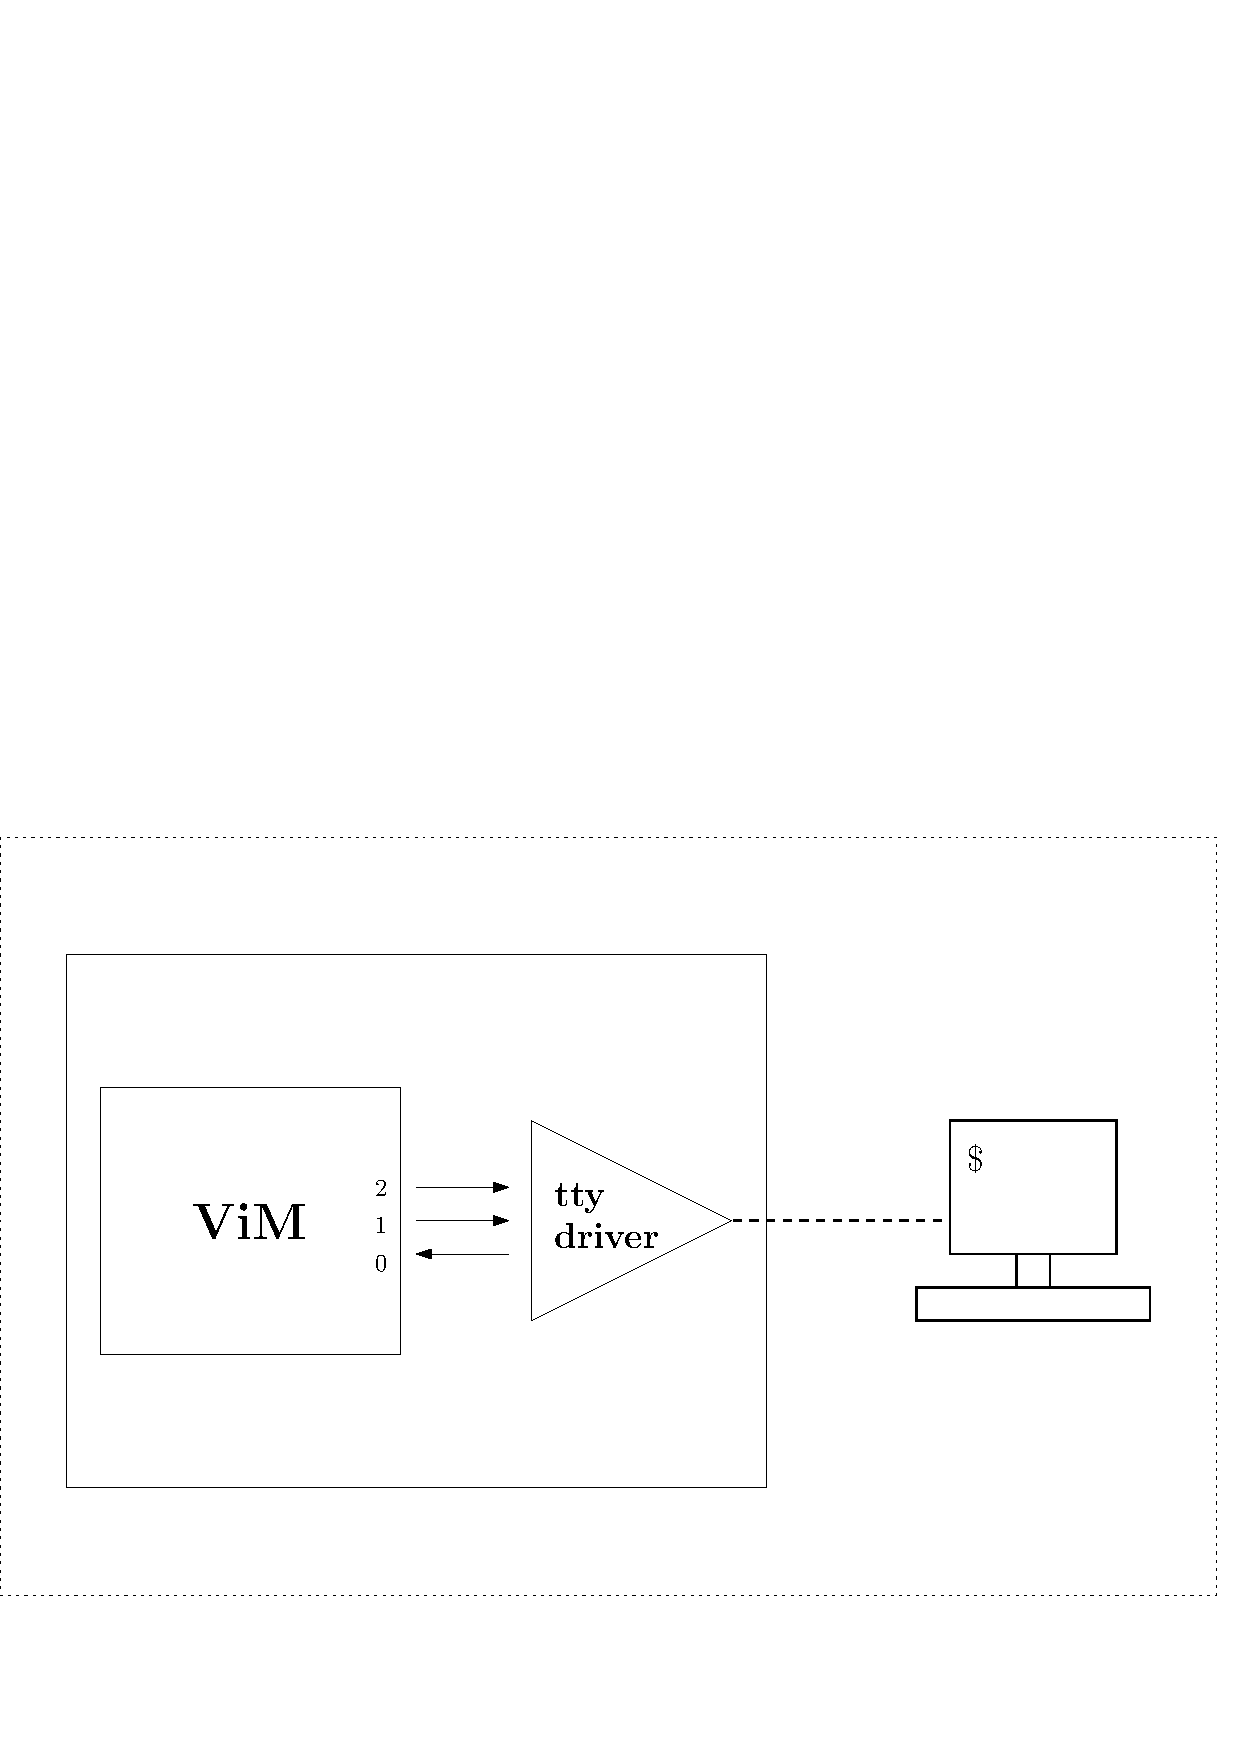
\includegraphics[width=105mm]{img/terminals/working-with-phy-term.pdf}
\end{center}

\begin{itemize}
\item The ViM editor communicates with the terminal driver, the driver takes
care of the communication with the actual physical terminal.
\item This is how it also looks when you run ViM from the virtual console.
\end{itemize}

%===============================================================================
\subsection{Pseudo terminals Overview}

\begin{itemize}
\item pseudo terminal is an emulation of a physical terminal
\item \emsl{allows one process to control another process that is written for a
terminal}
\begin{itemize}
	\item remotely running ViM over an SSH connection, for example
	\item such application (SSH) must support it in order this can work
\end{itemize}
\item you can have multiple (text) terminals on your desktop
\item an application written for a terminal does not care (more or less) whether
it communicates with a physical or a pseudo terminal
\end{itemize}

\begin{itemize}
\item The pseudo terminal device driver acts just like a terminal as far as the
interactive (slave) process is concerned. However, the other end is connected to
a master process, not to the physical device. The master process can read from
the pty master what the application wrote to it, and can write to the pty master
what it wants the application to read from the slave pty.
\item In other words, the master side of the pseudo terminal represents the
physical terminal, the slave part represents the special device end point.
\item The pseudo terminal can not be just one point used by both processes. It
is the same as a (bidirectional) pipe - you need 2 ends so that the processes
can communicate with each other.
\end{itemize}

%===============================================================================
\subsection{PTY Driver Connected To a Process}

\begin{center}
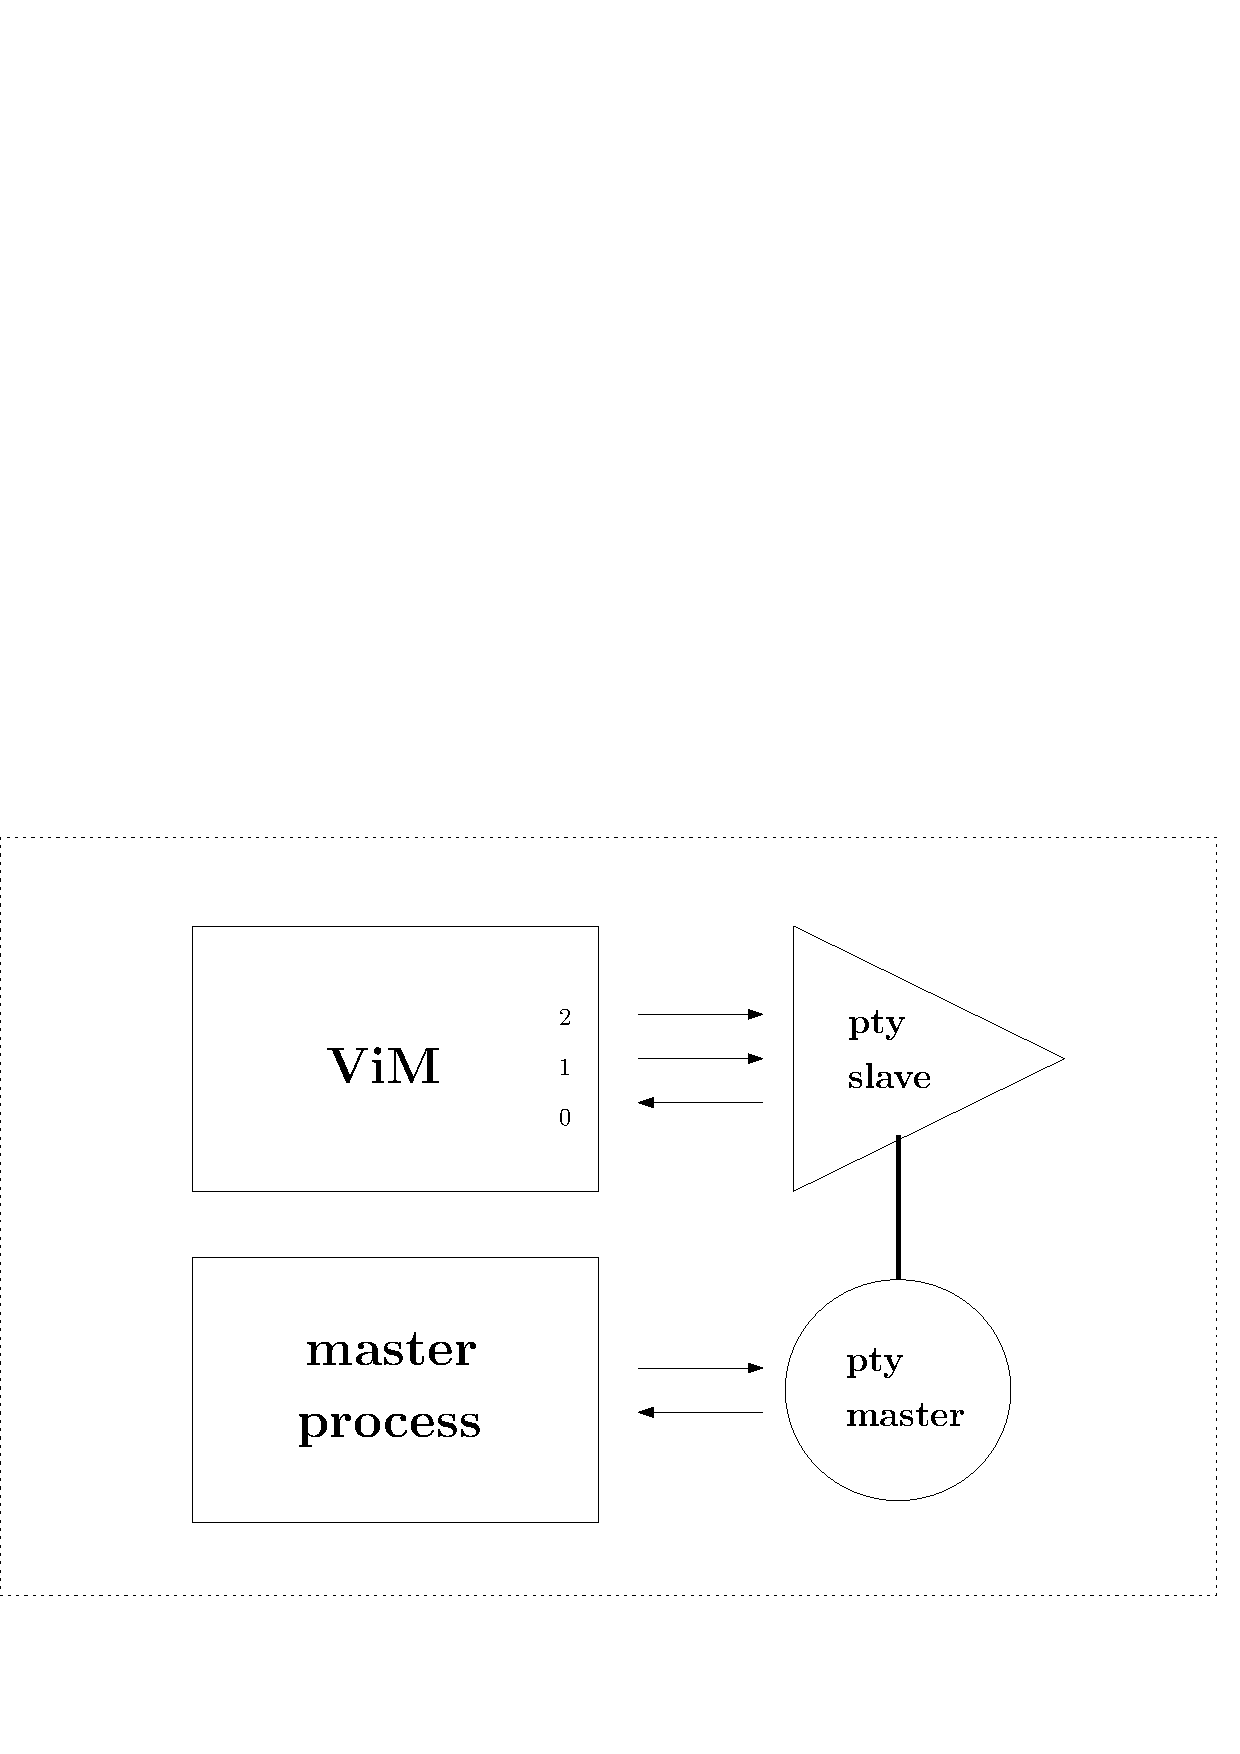
\includegraphics[width=105mm]{img/terminals/working-with-pty.pdf}
\end{center}

\begin{itemize}
\item The master process can be \texttt{xterm}, for example, running a shell
which started the ViM editor. More processes can work with the same terminal, as
we will see later.
\item \emsl{The master process and the master PTY together emulates the physical
terminal.}
\item How to get the pseudo terminal and how to use it in your program will be
explained later in the chapter.
\item How exactly is the slave and the master part ``connected'' together in the
kernel does not have to be of a programmer's concern.
\end{itemize}

%===============================================================================
\subsection{More Complex Example}

\begin{center}
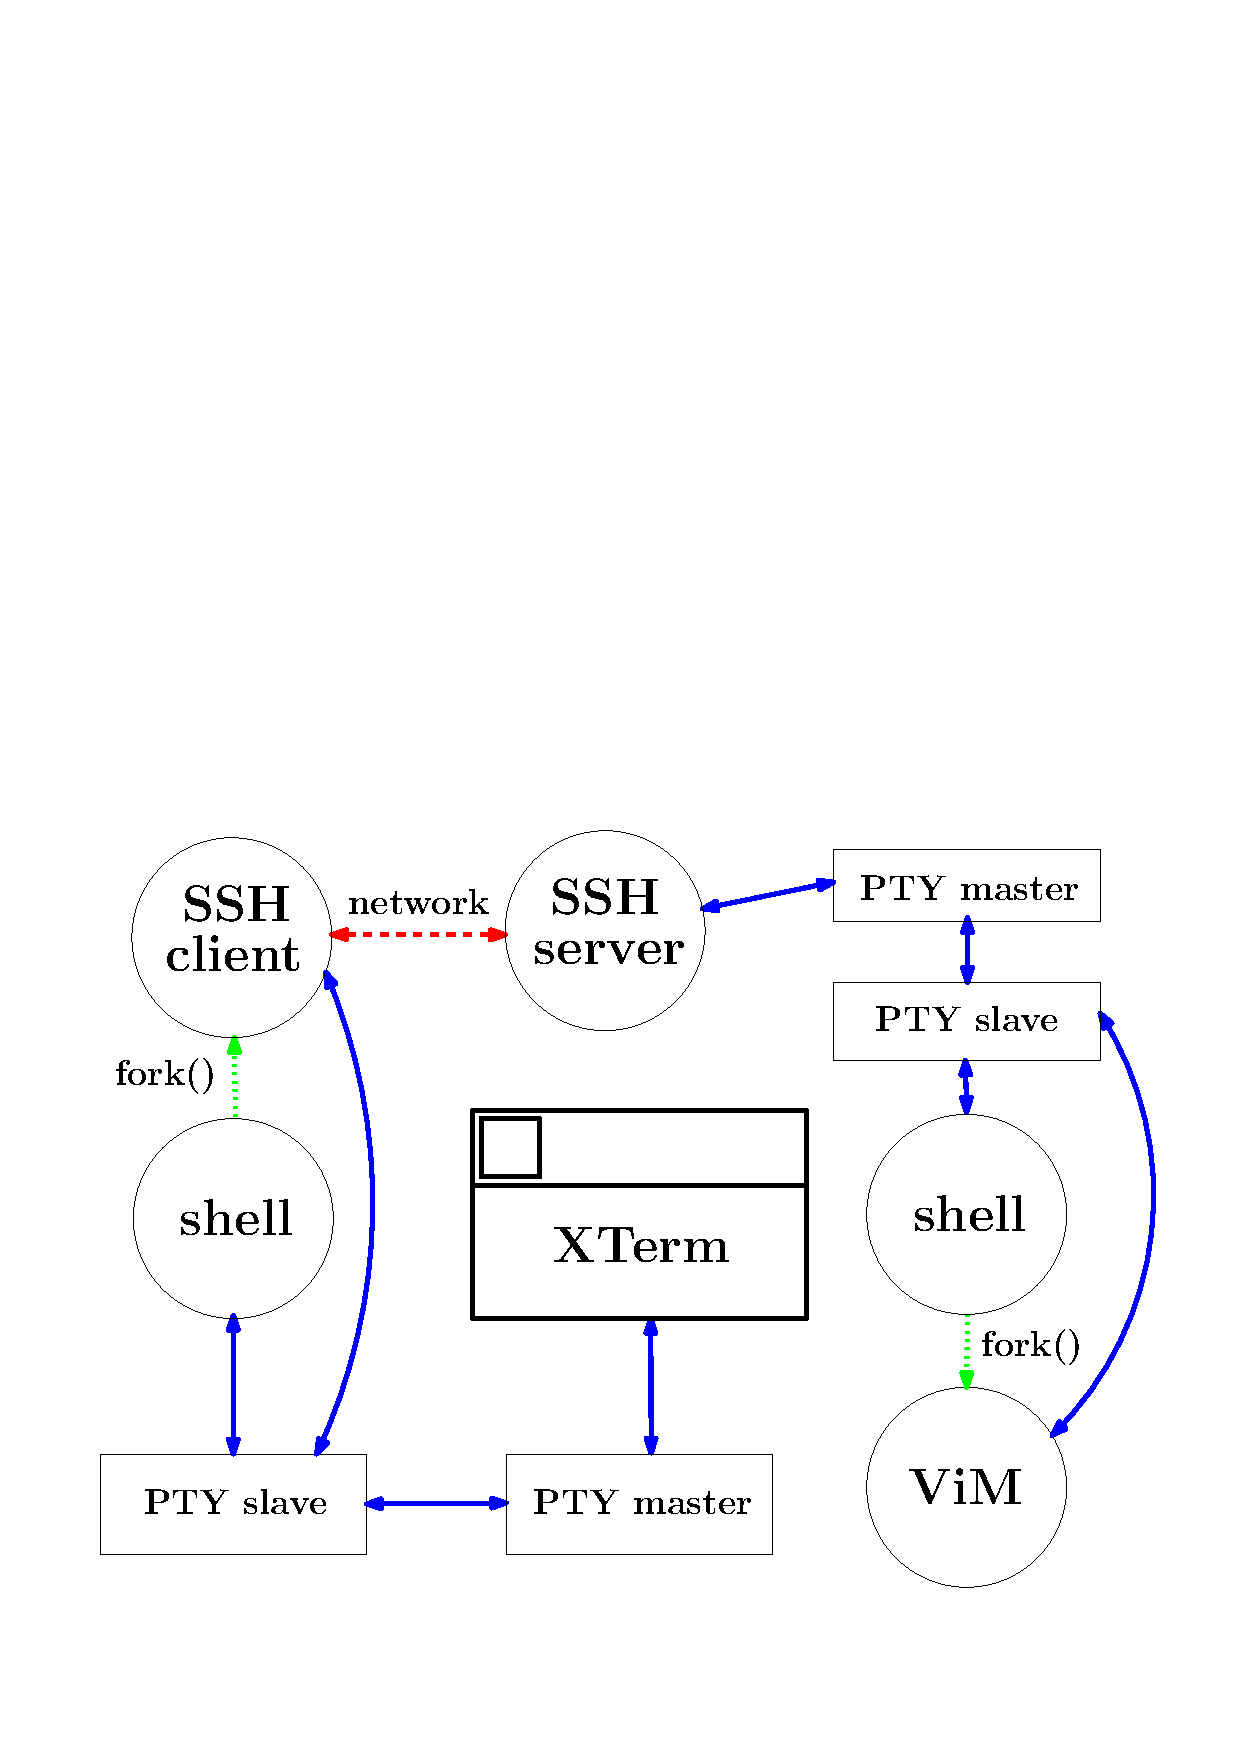
\includegraphics[width=90mm]{img/terminals/remote-vim-with-pty.pdf}
\end{center}


\begin{itemize}
\item The picture shows a situation where an SSH client running from a shell in
a terminal window is connected to the remote side, and running ViM there.
\item Note that ViM is not communicating over the shell. It is reading and
writing to the same terminal as the shell is. It is about process groups and
the controlling terminal as we will see later in the chapter.
\item The communication between the 2 pseudo terminal ends is bidirectional (in
other words, it's full duplex).
\item Question: when user runs ViM over SSH, what is the settings of the slave
pseudo terminal devices on remote and local side?
	\begin{itemize}
	\item Answer: will be the same because SSH transmits all terminal
	settings to the other side, see RFC 4254 above.
	\end{itemize}
\item Example:

\begin{verbatim}
# Get the local pseudo terminal name, remotely log in using
# SSH, get the remote pseudo terminal name there as well,
# and then run ViM.
$ tty
/dev/pts/5
$ ssh localhost
Password: 
$ tty
/dev/pts/8
$ vim 

# And now from another console, check the settings of both
# slave pty's.
$ /usr/gnu/bin/stty --file=/dev/pts/5
speed 38400 baud;
eol2 = M-^?; swtch = <undef>; min = 1; time = 0;
-icrnl
-opost
-isig -icanon -iexten -echo -echoe -echok

$ /usr/gnu/bin/stty --file=/dev/pts/8
speed 38400 baud;
eol2 = M-^?; swtch = <undef>; min = 1; time = 0;
-icrnl ixany
-onlcr tab3
-isig -icanon -iexten -echo -echoe
\end{verbatim}

\end{itemize}

%===============================================================================
\subsection{Reading From a Terminal}

\begin{itemize}
\item normally, the application uses descriptors 0, 1, and 2
\begin{itemize}
	\item those may or may not be connected to a terminal
	\item if not, user probably redirected those, eg.\\
	\texttt{cat /etc/passwd > my\_passwd}
\end{itemize}

\item an application can explicitly open \texttt{/dev/tty}
\begin{itemize}
	\item a synonym for a controlling terminal for the process
	\item the reason to do that might be to read a password and bypassing
	any redirections
\end{itemize}
\item an app can (try to) open actual terminal name (eg., \texttt{/dev/tty02})
\end{itemize}

\begin{itemize}
\item Applications usually do not allow to read a password from a redirected
file for security reasons. However, they might provide a way to do it via a
separate program. For example, look for \texttt{SSH\_ASKPASS} in \texttt{ssh(1)}
manual page.
\item See \priklad{terminals/getpassphrase.c}, read the comment inside. The
program will use the terminal no matter how you redirect the standard input.
And, if you have no terminal at all, it will fail the way as documented in
the manual page for \texttt{getpassphrase(3C)}.
\item Shell command \texttt{tty(1)} prints the controlling terminal:

\begin{verbatim}
$ tty
/dev/pts/15
$ pfiles $$
2256:   bash
  Current rlimit: 256 file descriptors
   0: S_IFCHR mode:0620 dev:342,0 ino:453881557 uid:1629480 gid:7 rdev:24,15
      O_RDWR|O_NOCTTY
      /dev/pts/15
   1: S_IFCHR mode:0620 dev:342,0 ino:453881557 uid:1629480 gid:7 rdev:24,15
      O_RDWR|O_NOCTTY
      /dev/pts/15
   2: S_IFCHR mode:0620 dev:342,0 ino:453881557 uid:1629480 gid:7 rdev:24,15
      O_RDWR|O_NOCTTY
      /dev/pts/15
   3: S_IFDOOR mode:0444 dev:351,0 ino:50 uid:0 gid:0 size:0
      O_RDONLY|O_LARGEFILE FD_CLOEXEC  door to nscd[328]
      /var/run/name_service_door
 255: S_IFCHR mode:0620 dev:342,0 ino:453881557 uid:1629480 gid:7 rdev:24,15
      O_RDWR|O_NOCTTY FD_CLOEXEC
      /dev/pts/15
\end{verbatim}
\end{itemize}

%===============================================================================
\subsection{Reading From a Terminal (cont.)}

\begin{itemize}
\item normally, an application gets input in lines because the terminal driver
does not send the data up until ``Enter'' is hit.
\begin{itemize}
	\item unless the input/output is redirected to/from a non-terminal
\end{itemize}
\item no arrow keys, deletes, backspaces get through to the application. All
that is handled in the driver.
\begin{itemize}
	\item it is said that terminal is in the \emph{canonical mode}
\end{itemize}
\item Ctrl+D at the beginning of the line means ``End of File''. \texttt{read()}
then returns 0 to indicated it.
\end{itemize}

\begin{itemize}
\item For more information on terminal modes, see page \pageref{CANONICAL}.
\item See examples (again, read the comments):
\priklad{terminals/simple-read.c} and
\priklad{terminals/simple-tty-read.c}. The 2nd one does similar thing to what
\texttt{getpassphrase(3C)} does. Try without a terminal to see that.
\item \texttt{O\_NONBLOCK} can be used as usual. Either with \texttt{fcntl()} on
the file descriptor, or directly with \texttt{open()} in which case it also
affects \texttt{read()} as well. See [\myun\myix-prog] for more info.
\item Do not forget that \texttt{select()} and \texttt{poll()} calls are useful
when there is a need to read from more file descriptors without busy waiting.
\end{itemize}

%===============================================================================
\subsection{Sessions and Process Groups (Jobs)}

\begin{itemize}
\item a new \emph{session} is created when the user logs in
\item that new session consists of one \emph{process group}
\item the only process in the process group is the login shell
\begin{itemize}
	\item that is the simple scenario with no windowing environment
\end{itemize}
\item the process is a \emph{process group leader} and a \emph{session leader}
as well
\begin{itemize}
	\item its PID is also a proces group ID and a session ID
\end{itemize}
\item that's how it is today. The history of this was quite colorful and
diverse.
\end{itemize}

\begin{itemize}
\item Some of that was in [\myun\myix-prog].
\item Example to show that my login shell is both the session leader and a
process group leader ("-j" prints session and process group ID as well):

\begin{verbatim}
$ ssh $(hostname)
Password: 

$ ptree $$
503   /usr/lib/ssh/sshd
  4117  /usr/lib/ssh/sshd
    4118  /usr/lib/ssh/sshd
      4124  -bash
        4160  ptree 4124
$ ps -j -p 4124
  PID  PGID   SID TTY         TIME CMD
 4124  4124  4124 pts/10      0:00 bash
\end{verbatim}
\item The pseudo terminal slave, ie. the end used the by the terminal
application (\texttt{bash}), is \texttt{/dev/pts/10}.
\item And, if we use \texttt{pfiles} on the right \texttt{sshd} process, we can
see that the pty master end of the pseudo terminal is also 10 (note
``\texttt{rdev:23,10}'').

\begin{verbatim}
  11: S_IFCHR mode:0000 dev:341,0 ino:56712 uid:0 gid:0 rdev:23,10
      O_RDWR|O_NONBLOCK|O_NOCTTY|O_LARGEFILE
      /devices/pseudo/clone@0:ptm
\end{verbatim}
\item Remember that you can kill a process group with \texttt{kill(2)} by using
a negative number where the number is a process group PID. You can do the same
with \texttt{kill(1)} command: ``\texttt{kill -- -<PGPID>}''. Note that you must
not forget to use ``\texttt{--}'' to stop the command to interpret the process
group PID as an option. Killing the whole process group may come in handy if you
want to kill a big process group like a parallel system build with tens of
processes, etc.
\item \label{BASH_KSH} Try to run ``\texttt{sleep 991 | sleep 992 | sleep 993 |
sleep 994}'' and play with this process group. You can kill it as a group using
the negative number, you can try to kill individual process and see what
happens. Examining the behaviour of \texttt{bash}, for example, it will not
notify you that the job has finished until all processes of the group have
finished. Korn Shell 93 (\texttt{ksh93}), on the other hand, waits on the last
process only. You can also observe that there is a difference in how processes
are created. \texttt{bash} is the father of all processes and starts creating
those from left to right, Korn shell creates the last process in the pipe line
and all other processes in the job are created by it. Given that Korn shell
creates just one process, the group leader, it must create the last one in the
pipe since that assures that shell will wait for the whole pipe to get
completed.
\item \emsl{Exercise:} use Bash and Korn shell with the ``sleep'' job above and
verify the above mentioned information. With the Korn shell, use
\texttt{/bin/sleep} instead of \texttt{sleep} since the latter is a built-in
command in KSH so you would see only \texttt{ksh} in the process listing.
However, you need the seconds to distinguish between individual processes.
\end{itemize}

%===============================================================================
\subsection{Sessions and Process Groups (cont.)}

\begin{itemize}
\item the terminal the user logged in becomes a \emph{controlling terminal} of
the session
\item the session leader is also a \emph{controlling process}
\item if \emph{job control} is enabled, every command or a pipeline forms a new
process group
\begin{itemize}
	\item all such groups have the same controlling terminal, unless the
	application explicitly changes that
\end{itemize}
\end{itemize}

\begin{itemize}
\item See this commented output:
\begin{verbatim}
# Let's see what is in our process tree.
$ ptree $$
503   /usr/lib/ssh/sshd
  4117  /usr/lib/ssh/sshd
    4118  /usr/lib/ssh/sshd
      4124  -bash
        4283  ptree 4124

# Let's run the 1st job, on the background.
$ while true; do sleep 1; echo X; done | wc -l &
[1] 4291

# Let's run the 2nd job, on the background as well.
$ sleep 999 &
[2] 4303

# Let's see what jobs we have.
$ jobs
[1]-  Running   while true; do sleep 1; echo X; done | wc -l &
[2]+  Running   sleep 999 &

# Now, let's see our process tree again.
$ ptree $$
503   /usr/lib/ssh/sshd
  4117  /usr/lib/ssh/sshd
    4118  /usr/lib/ssh/sshd
      4124  -bash
        4290  -bash
          4316  sleep 1
        4291  wc -l
        4303  sleep 999
        4317  ptree 4124

# The following bash process is the process group leader for
# the while loop (note that 'while' is a shell internal
# command so that's why we see 'bash', not 'while' there).
# Also note that all those processes share the same login
# session, with session ID 4124.
$ ps -j -p 4290
  PID  PGID   SID TTY         TIME CMD
 4290  4290  4124 pts/10      0:00 bash

# Note that 'wc' is a member of the above mentioned process
# group as well and it is NOT a process group leader (bash
# with PID 4290 is).
$ ps -j -p 4291
  PID  PGID   SID TTY         TIME CMD
 4291  4290  4124 pts/10      0:00 wc

# However, 'sleep 999' was run as its own job so it formed a
# new process group, with one process in it (sleep) and
# sleep is the process group leader as well. You can also
# see that from the ptree(1) output that we cannot assign
# the commands listed to their respective groups, we must
# use ps(1) to get that additional information.
$ ps -j -p 4303
  PID  PGID   SID TTY         TIME CMD
 4303  4303  4124 pts/10      0:00 sleep
\end{verbatim}
\end{itemize}

%===============================================================================
\subsection{Controlling Terminal}

\begin{itemize}
\item a session can have one controlling terminal. Daemons usually do not have
it.
\item it is the \emsl{first terminal} that a session leader (and a session
leader \emsl{only} can do that) opens after the new session was created
\item the session leader that establishes the connection to the controlling
terminal is called a controlling process
\item terminal input and terminal generated signals go to the foreground group
only
\item if modem (or network) disconnect is detected by the terminal interface,
\texttt{SIGHUP} is sent to the controlling process or group
\end{itemize}

\begin{itemize}
\item A new session is created via calling \texttt{setsid(2)}, see
p\pageref{SETSID}.
\item As to differences between systems and the \texttt{SIGHUP} signal, see
p\pageref{SIGHUP_SIGNAL}.
\item The above says that there are sessions without a controlling terminal,
those sessions usually contain daemons, server processes, etc.
\item The above also says that in order to get rid of a controlling terminal,
you have to create a new session. It is not enough to close the controlling
terminal -- which would usually mean to close stdin, stdout, and stderr. See
\priklad{terminals/close-the-tty.c}. And, if you want to make sure you will
never get a controlling terminal in the session, let the session leader fork and
exit. Since only the session leader can acquire the controlling terminal, and we
have no session leader anymore (just its child), we are safe. Actually, that's
how the \texttt{daemon} call usually works.
\item If the session leader opens a terminal with \texttt{O\_NOCTTY}, such
terminal will not become the controlling terminal.
\item You cannot open \texttt{/dev/tty} to get a controlling terminal,
\texttt{/dev/tty} is a synonym for an already existing controlling terminal.
%\item TODO maybe a similar picture to the one in 9.6 (pic 9.7) of Adv Prog in
%UNIX (Stevens) could be included?
\item How to check that if you Ctrl-C your application the signal will go to the
foreground group and not to the shell? That's easy, get the PID of the shell,
run ``\texttt{sleep 999}'', run ``\texttt{truss -p <PID>}'' on the shell, and
then \^{}C the \texttt{sleep} process. You will see that the shell will get
\texttt{SIGCLD}, not \texttt{SIGINT}.
\item \emsl{Exercise:} write a very simple \texttt{tty} program. Read what
exactly \texttt{tty(1)} does and then use \texttt{truss} to find out what
function to call. It's basically a one-liner. The solution is in
\priklad{terminals/tty.c}.
\end{itemize}

%===============================================================================
\subsection{Job Control}

\begin{itemize}
\item the fact that a process group runs in the background does not mean that it
cannot use the terminal
\begin{itemize}
  	\item however, it can only write to it, cannot read from it
\end{itemize}
\item the "job control" means that certain signals are only sent to the
foreground process group
\begin{itemize}
	\item \texttt{SIGINT} (\texttt{\^{}C}), \texttt{SIGQUIT} (usually
	\texttt{\^}{}$\backslash$, quits and generates a core dump), and
	\texttt{SIGTSTP} (usually \texttt{\^{}Z}, suspends the process)
\end{itemize}
\item the "control" part of job control means that we can move jobs back and
forth between foreground and background, kill them independently of other jobs,
etc.
\item job control as such needs a system support for process groups
\end{itemize}

\begin{itemize}
\item The \emph{foreground process}, or the \emph{foreground group} if there are
more than one process in the group, is defined as process or a group that has an
unlimited access to the controlling terminal.
\item The \emph{controlling group} is a group associated with the terminal. If
job control is enabled, it's the same as the foreground group.
\item Every shell may do that differently but usually internal commands for job
control are "jobs", "fg", and "bg". Also, internal "kill" command can work with
job IDs. See manual page for your shell.
\item See the following bash example on \texttt{kill} shell internal command:
\begin{verbatim}
$ sleep 999 &
[1] 5760
$ jobs
[1]+  Running                 sleep 999 &
# use '%' with the job ID to kill a specific job
$ kill %1
[1]+  Terminated              sleep 999
\end{verbatim}
%\item TODO Put here what the shell does when putting a process to the
%foreground/background.
\end{itemize}

%===============================================================================
\subsection{What Happens If Job Control is Disabled?}

\begin{itemize}
\item in other words, how it was before job control was introduced...
\item you can still run processes in the background
\begin{itemize}
	\item but it means that the shell just does not wait for them
\end{itemize}
\item all processes are part of the same process group as the login shell
\item signals are sent to all processes
\item note that choosing a job control might be a compile time option of your
shell
\begin{itemize}
	\item bash has it like that
\end{itemize}
\end{itemize}

\begin{itemize}
\item Note that when bash is built with "\texttt{configure
--disable-job-control}" (which is not the default setting, obviously), all
commands started in the background will be spawned with \texttt{SIGINT} and
\texttt{SIGQUIT} ignored. That means that \^{}C will not kill them and will kill
only the pipeline in the foreground. That is what a user would most probably
expect. Killing background processes with \^{}C could really suprise the user.
\item \emsl{Exercise:} build Bash w/o the job control and verify the above
stated information. Use \texttt{psig} command on Solaris to see what signal
handlers are installed for commands started in the background.
\end{itemize}

%===============================================================================
\subsection{\texttt{SIGHUP} Signal}

\begin{itemize}
\item if the terminal hangs up or is disconnected, the controlling process
(shell) gets a \texttt{SIGHUP} signal (SVR4)
\begin{itemize}
  	\item or, the whole controlling group gets the signal (BSD)
\end{itemize}
\item usually, \texttt{SIGHUP} terminates the shell
\begin{itemize}
	\item in SVR4 though, the shell itself is expected to send
	\texttt{SIGHUP} to to \emsl{foreground group} before it exits
\end{itemize}
\item the shell \emsl{may} send \texttt{SIGHUP} to all processes in the session then
\begin{itemize}
	\item that's why you might need to start remote jobs with "\texttt{nohup
	<job>}" if you want them to survive the logout
	\item \texttt{ksh} and \texttt{bash} do that, not sure about other
	shells
\end{itemize}
\end{itemize}

\label{SIGHUP_SIGNAL}

\begin{itemize}
\item On Solaris, try the following. Start two \texttt{sleep} processes, one in
the foreground, one in the background:

\begin{verbatim}
$ echo $$
4104
$ sleep 888 &
[1] 4150
$ sleep 999
\end{verbatim}

and see how the process tree looks like from another terminal:

\begin{verbatim}
$ ptree 4104
...
...
  2659  /usr/local/bin/rxvt -fn fixed
      4104  bash
        4150  sleep 888
        4154  sleep 999
\end{verbatim}

Now, truss both \texttt{sleep} processes and the shell as well. When you kill
the terminal window which simulates the terminal disconnect, you will see that
the foreground \texttt{sleep} processes got \texttt{SIGHUP}s from the shell:

\begin{verbatim}
$ truss -p 4154
pause()                         (sleeping...)
    Stopped by signal #24, SIGTSTP, in pause()
    Received signal #15, SIGTERM, in pause() [default]
      siginfo: SIGTERM pid=4104 uid=1629480
pause()                                         Err#4 EINTR
\end{verbatim}

The \texttt{sleep} process in the background continues to run.
However, the shell gets the signal from the kernel (the terminal driver) since
there is no PID, and then it sent the signals to all existing process groups:

\begin{verbatim}
$ truss -p 2881
waitid(P_ALL, 0, 0x08047AA0, WEXITED|WTRAPPED|WSTOPPED|WCONTINUED) (sleeping...)
    Received signal #1, SIGHUP, in waitid() [caught]
...
...
kill(-2716, SIGHUP)                             = 0
kill(-2735, SIGHUP)                             = 0
\end{verbatim}

\item Note that there is a difference between a shell getting a \texttt{SIGHUP}
or a shell exiting. For example, if \texttt{bash} exits, it sends a
\texttt{SIGHUP} to the controlling group only (if you type \texttt{exit}, the
controlling group would be empty since no foreground process is running).
However, if you set the \texttt{huponexit} option; it sends \texttt{SIGHUP} to
all processes. You can verify it easily -- start \texttt{sleep 888} in the
background, truss it from another terminal, and exit the shell. The terminal
window disappears but the \texttt{sleep} process continues to run without
getting any signal.

\item There are significant differences between systems, expecially between
older systems, about how they deal with terminals, process groups, and such.
\item SVR3 (1986)
\begin{itemize}
	\item the session usually consisted of 1 process group, and terminal
	could be associated with only one group. Thus, if a new group was
	created, the (new) process leader was disconnected from the controlling
	terminal and had to open another one.
	\item however, it could still use it through already open file
	descriptors, no \texttt{SIGHUP} would be sent on death of the leader
	though (see below).
	\item also, process group could not close the controlling terminal and
	later allocate another one (screen(1) would not work there)
	\item on death of the group leader the kernel sends \texttt{SIGHUP} to
	all processes in the group, those processes lose the terminal and also
	the group ceases to exist (group ID of the processes is zeroed out)
	\item when the terminal is disconnected the driver sends \texttt{SIGHUP}
	to all processes in the session
	\item no job control possible		  	
	\item many other differencies from what we are used to today
\end{itemize}

\item 4.3BSD (1986)
\begin{itemize}
	\item a process can change its group ID
\begin{itemize}
		\item thus we can have process groups without a leader
\end{itemize}
	\item more groups can share the same controlling terminal
\begin{itemize}
		\item but the terminal can control just one group
\end{itemize}
	\item background process gets \texttt{SIGTTIN} on read (will suspend it
	by default)
	\item background process can write to a terminal (or get
	\texttt{SIGTTOUT} if the terminal is configured that way)
	\item when the terminal is disconnected the driver sends \texttt{SIGHUP}
	to the controlling group (only)
	\item on session end, \texttt{vhangup()} is used on the controlling
	terminal to traverse the process table, all the terminal entries are
	made unusable, then it \texttt{close()} the terminal, and
	\texttt{SIGHUP} is sent to the controlling group.
\begin{itemize}
		\item that's why on, for example, FreeBSD all background
		processes survives the logout.
\end{itemize}
	\item however, there is no notion of a controlling process as it was in
	SVR3.
\end{itemize}

\item SVR4 (1990)
\begin{itemize}
	\item have sessions and process groups
	\item controlling terminal is associated with a session and a foreground
	process group
	\item only session leader may allocate and deallocate a controlling
	terminal
\end{itemize}
\end{itemize}

%===============================================================================
\subsection{So called hang-on-exit problem}

\texttt{\$ ssh bash\_user@hostname "sleep 10 \&"}

\begin{itemize}
\item the above hangs for 10 seconds on Solaris and Linux
\item however, it does not on FreeBSD, OpenBSD, and NetBSD
\begin{itemize}
	\item in both cases though, the shell itself exits immediatelly
	\item so, why the hang?
\end{itemize}

\item SSH sleeps in \texttt{select()}, waiting on an event on the terminal
\begin{itemize}
	\item and on Solaris and Linux, it does not get the end-of-file when the
	shell exits. See notes for more info.
\end{itemize}

\item bash's \texttt{huponexit} prevents the hang on Solaris and Linux but for
the price of \texttt{SIGHUP} killing the process
\end{itemize}

\begin{itemize}
\item On BSD, \texttt{revoke()} is used to revoke all descriptors using the
terminal, and SSH daemon thus gets 0 (end-of-file) on \texttt{read()}. And,
\texttt{sleep(1)} still runs after the connection closes.
\item On Solaris and Linux, that does not happen since there is no
\texttt{revoke()}, so the \texttt{sleep(1)} command keeps the terminal open
which is why the SSH daemon does not get end-of-file till \texttt{sleep(1)}
exits.
\item You should definitely try it yourself on those systems.
\item See a discussion on OpenSSH mailing list. Look for
"so-called-hang-on-exit" and especially for the subject "The complete answer
(was Re: so-called-hang-on-exit)" by Nico Williams; it has a lengthy
explanation of the problem:\\
\url{http://marc.info/?l=openssh-\myun\myix-dev&m=102878253003241&w=2}
\item On Solaris:
\begin{verbatim}
$ ssh localhost
$ sleep 99 &
[1] 4552
$ logout
<HANGS HERE UNTIL THE SLEEP CMD EXITS>
\end{verbatim}

However, if you use the \texttt{huponexit} option in \texttt{bash}:

\begin{verbatim}
$ ssh localhost
$ shopt -s huponexit
$ sleep 99 &
[1] 4552
$ logout
Connection to localhost closed.
\end{verbatim}
\end{itemize}

%===============================================================================
\subsection{Function calls for sessions and process groups}

\texttt{int \funnm{setsid}(void);}
\begin{itemize}
\item creates a new session, with the current process as a session leader
\end{itemize}
\texttt{int \funnm{setpgid}(pid\_t \emph{pid}, pid\_t \emph{pgid});}
\begin{itemize}
\item sets the process group ID \texttt{pgid} for process \texttt{pid}
\end{itemize}
\texttt{int \funnm{getsid}(pid\_t \emph{pid});}\\
\texttt{int \funnm{getpgid}(pid\_t \emph{pid});}
\begin{itemize}
\item get the session or process group ID of process with PID \texttt{pid}
\end{itemize}

\begin{itemize}
\item \label{SETSID} The process calling \texttt{setsid} must not be a process
group leader. \texttt{EPERM} is returned otherwise.
\item New session has no controlling terminal. That's perfect for daemons since
they do not need any.
\item Normally, you can use \texttt{daemon()} call to daemonize your app which
does the right thing. It might not be available on your system so the way how to
do it is this:
	\begin{itemize}
	\item fork()
	\item the parent exits
	\item the child calls setsid()
	\item and redirects 0/1/2 file descriptors from/to \texttt{/dev/null}
	(ie., it opens \texttt{/dev/null}, \texttt{dup2()} it to 0/1/2, and
	closes it again).
	\end{itemize}
\item Source code example: \priklad{terminals/daemonize.c}.
\end{itemize}

%===============================================================================
\subsection{Opening a Terminal}

\begin{itemize}
\item On a classic terminal login each configured terminal is managed by
\texttt{init}, followed by \texttt{getty} and \texttt{login}.
	\begin{itemize}
	\item And \texttt{getty} is run with the terminal name as a parameter so
	it knows which terminal to open. It initializes the line, reads the user
	name and \texttt{exec()}s \texttt{login} with the username as a
	parameter.
	\end{itemize}

\item On networks logins and on terminals that are run through your windowing
environment, pseudoterminals are used.
	\begin{itemize}
	\item You ask for a new pseudoterminal then. More on that soon.
	\end{itemize}

\end{itemize}

\begin{itemize}
\item By classic terminal login we mean sitting in front of a black screen with
"Login:" only.
\item By configured terminals we mean even virtual terminals used usually via
Alt-Fxx keys from the text console.
\end{itemize}

%===============================================================================
\subsection{Working with Pseudoterminals}

\begin{itemize}
\item different on different systems
\item however, POSIX defines functions that should be used
	\begin{itemize}
	\item systems map their native calls to POSIX calls:
	\end{itemize}
\end{itemize}

\begin{verbatim}
posix_openpt() - open a master pseudo terminal device
grantpt()      - changes the ownership of the corresponding
                 slave device to the calling UID
unlockpt()     - unlock the corresponding slave device so
                 that it can be read/written from/to
ptsname()      - gets the name of the corresponding slave
                 device
\end{verbatim}


\begin{itemize}
\item \texttt{xterm} uses \texttt{posix\_openpt()}, \texttt{grantpt()}, and
\texttt{unlockpt()}.
\item \texttt{xterm} forks, calls \texttt{pstname()} to get the slave device,
and redirects 0/1/2 to the slave for the child.
\item xterm's child \texttt{exec()}s the shell.

\item For example, Linux gets the master pseudo terminal by calling
\texttt{getpt(3)}, Solaris by opening \texttt{/dev/ptmx} etc.
\texttt{posix\_openpt()} is then implemented by those native function calls.

\item On Solaris, the app needs to push \texttt{ptem} and \texttt{ldterm}
modules onto the slave side to get terminal semantics.
	\begin{itemize}
	\item pty's are implemented using STREAMS on Solaris
	\item see the example code
	\end{itemize}
\item Source code example on how one process can communicate with another
process over a newly allocated pseudo terminal: \priklad{terminals/pty.c}.
\end{itemize}

%===============================================================================
\subsection{Setting Terminal Attributes}

\begin{itemize}
\item various terminal attributes can be set
	\begin{itemize}
	\item terminal speed, uppercase to lowercase conversion, remapping
	various control characters, echo switch off/on, etc.
	\end{itemize}
\item \funnm{tcgetattr}(), \funnm{tcsetattr}()
\item canonical versus punctual mode
	\begin{itemize}
	\item normally, input characters are queued until a line is complete, as
	indicated by pressing an Enter
	\item in the punctual mode, there is no line queing.
	\end{itemize}
\item raw mode is punctual with many other attributes switched off, including
ECHO
	\begin{itemize}
  	\item editors usually operate in raw mode
	\end{itemize}
\end{itemize}

\label{CANONICAL}
\label{TERMIOS}

\begin{itemize}
\item The terminal attributes are set using the \texttt{termios} structure that
is used as a parameter of a subsequent \texttt{tcsetattr()} call. The structure has
input (eg. enable start/stop input control), output (eg. map CR to NL on
output), control, and local modes (eg. enable echo on/off). Then it has an array
of control characters (EOF, INTR, START, STOP, SUSPEND, ...) mapped to
characters  -- usually \^{}D, \^{}C, \^{}Q, \^{}S, \^{}Z, respectively.
\item So, if you want to be able to generate EOF with \^{}X instead of \^{}D,
you would use ``\texttt{stty eof \^{}X}''. \texttt{stty(1)} would change
\texttt{termios.c\_cc[VEOF]} to \texttt{24} and then set the new structure via
\texttt{tcsetattr()} with command \texttt{TCSANOW} (Change Attributes Now), for
example. See \texttt{termios.h} in the UNIX spec for more information on all
required terminal control characters.
\item Raw mode with no ECHO is used when you type a password, for example,
and want to print * for every character typed. You could not do that in the
canonical mode. See the \texttt{ICANON} flag in \texttt{c\_lflag} of the
\texttt{termios} structure. Also, see \texttt{MIN} and \texttt{TIME} params. For
more information, consult manual page for \texttt{termio(7I)}.
\item There is no single attribute to set for the raw mode. See \texttt{-raw}
option in \texttt{stty(1)} man page for the list of attributes switched off/on
for that mode.
\item Some old terminals could print only uppercase. To input/output an
uppercase then, the letter is preceded by a backslash.
\item Example on how to switch the echo off: \priklad{terminals/no-echo.c}.
Note that it is independent on whether we use a physical terminal or a pseudo
terminal. That means that we work with the terminal driver which is the slave
part in case of pseudo terminals. That is the part that echos the characters
read from the terminal.
\item \emsl{Exercise:} you can modify the \texttt{no-echo.c} code so that you
can read the password and print * for each character typed. It's fine to ignore
all special characters like backspace, arrows, etc. You will have to switch off
the canonical mode and use \texttt{c\_cc} field of the \texttt{termio} structure
to set those \texttt{MIN} and \texttt{TIME} parameters. Hint -- when used as
indexes, you prepend \texttt{V} to them. Solution:
\priklad{terminals/type-password.c}. Read \texttt{termio} manual page for
more information.
\end{itemize}

%===============================================================================
\subsection{Terminfo database}

\begin{itemize}
\item a database describing the capabilities of devices such as terminals and
printers
\item devices are described by specifying a set of capabilities and character
sequences that trigger them
\item screen oriented apps (eg., \texttt{vim}) and other commands (eg.,
\texttt{ls}) use \emsl{generic} capabilities without a need to know the exact
terminal used
\item terminfo source files are converted into a database by the \texttt{tic}(1)
command
\item terminfo source files are usually in \texttt{/usr/share/lib/terminfo}
\end{itemize}

\begin{itemize}
\item Terminfo capabilities:
	\begin{itemize}
	\item Boolean capabilities
		\begin{itemize}
		\item Whether the terminal has the feature or not.
		\item Eg., can clear the screen.
		\end{itemize}
	\item Numeric capabilities:
		\begin{itemize}
		\item Quantifying a particular feature of a device.
		\item Eg., number of columns in a line
		\end{itemize}
	\item String capabilities:
		\begin{itemize}
		\item Providing sequences used to perform particular operations
		on devices.
		\end{itemize}
	\end{itemize}
\item terminfo is an System V equivalent of the original \emph{termcap} system
born in the BSD world. The termcap was invented by Bill Joy after he wrote the
first version of the \texttt{vi} editor. After the ininitial version of the
editor was written for a specific terminal, users started to want ports of the
editor for different terminals. Instead of bending the editor for each
available terminal, Bill Joy rewrote the editor with generic commands to
manipulate the terminal, and introduced a \emph{termcap} database containing
capabilities of various terminals, and a library to query the database.
\item termcap is a text based database, usually in \texttt{/etc/termcap}, see
FreeBSD, for example. It is just one file. Terminfo is a compiled database,
built from a separate files, one for each terminal. It might not come with the
source files used to build the database. On Solaris, it is in
\texttt{/usr/share/lib/terminfo}. It contains subdirectories named after letters
to accomodate hundreds of terminals in an easy way.
\item you can use \texttt{infocmp} to display the contents of the terminfo
entry:

\begin{verbatim}
$ infocmp vt100
#       Reconstructed via infocmp from file:
#       /usr/share/lib/terminfo/v/vt100
vt100|vt100-am|dec vt100 (w/advanced video),
    am, mir, msgr, xenl, xon,
    cols#80, it#8, lines#24, vt#3,
    acsc=``aaffggjjkkllmmnnooppqqrrssttuuvvwwxxyyzz{{||}}~~,
    bel=^G, blink=\E[5m$<2>, bold=\E[1m$<2>,
...
...
\end{verbatim}

\item For example, \texttt{am} means ``automargin'', ie. when a line reaches the
right edge of the screen, the terminal automatically continues on the next line.
\texttt{cols\#80} says that the terminal has 80 columns.
\item Example: move the cursor to the specified position when the terminal is
\texttt{xterm}. Solution is in \priklad{terminals/move-cursor-on-xterm.c}.
You can set \texttt{PS1} to an empty string to see that the cursor will get to
the absolute position then.
\item \emsl{Exercise:} clear the screen and then move the cursor to the
specified position on any supported terminal. Use low level terminfo routines to
do that. Those routines are beyond the scope of this lecture, read apropriate
documentation if you are interested. However, it is recommended to use
\emph{curses} which is a higher level interface. Anyway, the solution to
experiment with is here: \priklad{terminals/move-cursor-with-terminfo.c}.
\end{itemize}

\endinput
